\chapter[Appendix XX]{Appendix XX (supplementary to Chapters 2 and 3)}

\section{Study regions in Chapters 2-4}

%%%% FIGURE 1
\begin{figure}[ht]
\begin{center}
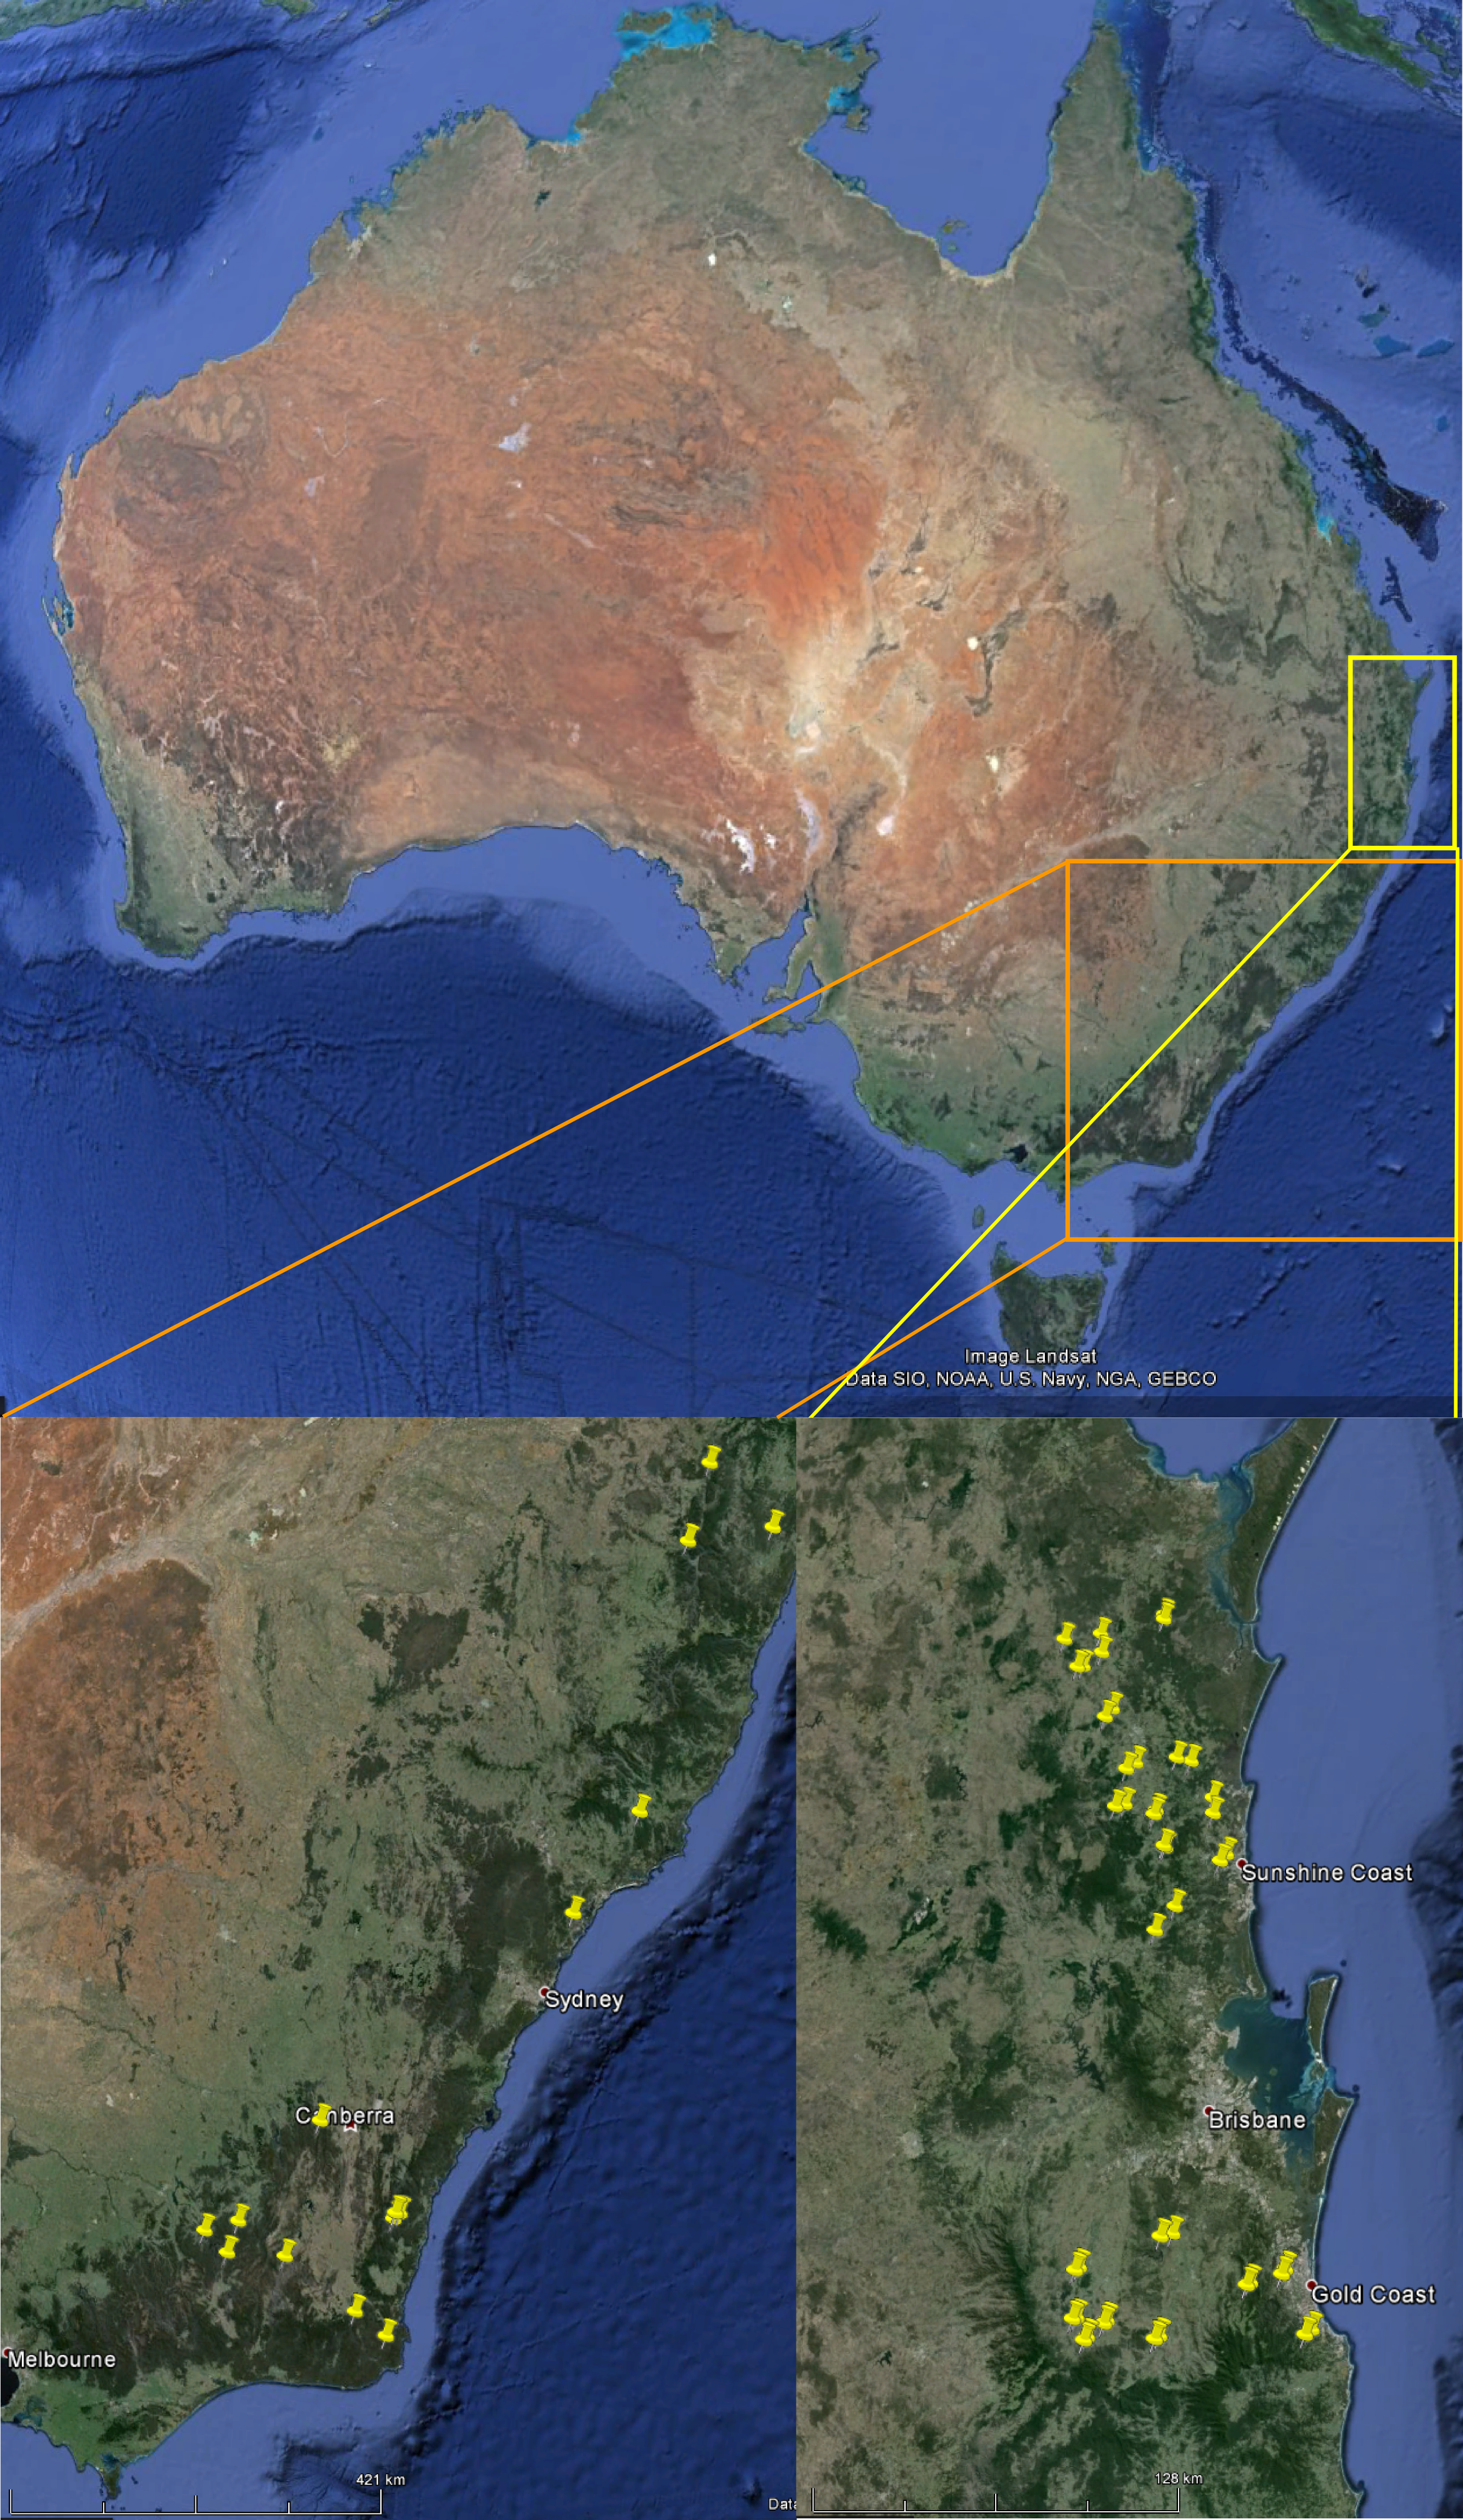
\includegraphics[width=12cm,keepaspectratio=true]{Ch6map.png} % figures can be in pdf, png, jpeg or eps format
\caption[Map of study areas described in Chapters 2-4.]{\small{Map showing study areas, and geographical distribution of field sites described in Chapters 2 \& 3 (lower left) and 4 (lower right) (Google Maps 2015).}\label{fig:Ch6_F1}}
%\label{Ch6_F1} % label for cross-referencing
\end{center}
\end{figure}   
\clearpage

\section{Biophysical characteristics of study sites}

This section describes the biophysical characteristics of study sites used in Chapters 2 and 3. For further information about study sites used in Chapter 4, the reader is referred to \citep{Arthington2012}.

\subsection{Biogeography}
koppen climate zone
ibra


\subsection{Catchment characteristics}

-	Catchment land use
-	Flow modification?
-	Distance from coast
-	Size?
-	Topography

\subsection{Fluvial geomorphology}

-	Valley extent and confinement
-	Substrate
-	Field sampling design?


\subsection{Vegetation}

-	Structure
-	Dominant species
-	In situ clearing / anthropogenic disturbance
-	Photos



